\section{Introduction}
A differential equation is an equation that contains derivatives. First order differential equations can be written as:
\[ \frac{dy}{dt} = f \pren{t, y} \text{ or } y \prime = f \pren{t, y} \]

Most differential equations have infinite solutions. The simplest differential equation is:
\[ \frac{dy}{dt} = f \pren{t} \]

The solution can be found through integration, yielding:
\[ y = \int f \pren{t} dt + c \]

Often we will need the solution that has a specified point $(t_0, y_0)$. We call these types of problems Initial Value Problems (IVP) where
\[ \frac{dy}{dt} = f \pren{t, y} \text{ and } y(t_0)=y_0 \]

An Equilibrium Solution is defined as a solution that doesn't change over time.
\begin{equation}\label{eq:EquilibriumSolution}
    \begin{aligned}
    y(t) = c \text{ and } y\prime(t) = 0\\
        \begin{cases}
        \text{Stable if solutions converge as } t \to \infty \\
        \text{Unstable if solutions diverge as } t \to \infty \\
        \text{Semistable if solutions converge in one direction, and diverge in the other}
        \end{cases}
    \end{aligned}
\end{equation}\myequations{Equilibrium Solution}

Differential Equations generally have a family of solutions, but Initial Value Problems usually only have one.

    \subsection{Visually Representing Differential Equations}\label{sec:visde}

    We can visually graph the solutions to a first order differential equation easily using direction fields. A direction field is a graph that shows the slope of the function at any given point.

    We can also use isoclines to determine the shape of the differential equation. An Isocline can be defined as a curve in the $t-y$ plane in which the slope is constant. In other words, wherever the slops has the value $c$.

\section{Seperation of Variables}
A separable differential equation can be written as:

\begin{equation}\label{eq:seperableeq}
y\prime = f(t)g(y)
\end{equation}\myequations{Separable Differential Equation}

    \subsection{Example}
    \[
    \begin{aligned}
        y\prime = 3t^2 (1 + y) \to \frac{dy}{dt} = 3t^2 (1 + y)\\
        \frac{dy}{1+y} = 3t^2 \to \int \frac{dy}{1+y} = \int 3t^2\\
        \ln\abs{1 + y} = t^3 + c \to \abs{1 + y} = e^c e^{t^3}\\
        y = c e^{t^3} - 1, \, k \ne 0
    \end{aligned}
    \]

\section{Approximation Methods}

Currently we can only solve a small subset of Differential Equations -- those that are separable \eqref{eq:seperableeq}. Typically it is not possible using this method to fin the solution $y=\Phi (t)$.

Recall that one meaning of ``solving'' a differential equation is to use a computer to approximate a solution at a specific set of time values. This leads us to Euler's Method.

    \subsection{Euler's Method (Tangent Line Method) - 1768}
    With a given function $y\prime = f(t,y)$ and a given set point $p_0$ we can approximate the line point by point.

    \begin{equation}\label{eq:eulersmethod}
    \begin{aligned}
    \text{For the initial value problem } y\prime = f(t,y), y(t_0) = y_0\\
    \text{Use the formulas }
    \begin{cases}
    t_{n+1} = t_n + h\\
    y_{n+1} = y_n + h f(t_n, y_n)
    \end{cases}
    \end{aligned}
    \end{equation}\myequations{Euler's Method for Approximate Solutions}

        \subsubsection{Example}
        \[
        \begin{aligned}
        \text{Obtain Euler approximation on }[0, 0.4] \text{ with step size } 0.1 \text{ of}\\
        y\prime = -2ty + t \text{ and } y(0) = -1\\
        h = 0.1, 
        \begin{cases}
        t_0 = 0\\
        y_0 = -1\\
        \end{cases} \\
        \to \begin{cases}
        t_1 = t_0 + h = 0.1\\
        y_1 = y_0 + h f(t_0, y_0) = -1
        \end{cases}\\
        \to \begin{cases}
        t_2 = t_1 + h = 0.2\\
        y_2 = y_1 + h f(t_1, y_1) = -0.97
        \end{cases}\\
        \to \begin{cases}
        t_3 = t_2 + h = 0.3\\
        y_3 = y_2 + h f(t_2, y_2) = -0.9112
        \end{cases}\\
        \to \begin{cases}
        t_4 = t_3 + h = 0.4\\
        y_4 = y_3 + h f(t_3, y_3) = -0.826528
        \end{cases}\\
        \end{aligned}
        \]
    \subsection{Runge-Kutta Method of Approximation}
    If we have an IVP, we can calculate the next values with a process similar to \eqref{eq:eulersmethod}

    \begin{equation}\label{eq:2ork}
    \begin{aligned}
    \begin{cases}
    t_{n+1} = t_n + h\\
    y_{n+1} = y_n + h k_{n2}
    \end{cases}\\
    \text{Where}\\
    k_{n1} = f(t_n, y_n)\\
    k_{n2} = f \left( t_n + \frac{h}{2}, y_n + \frac{h}{2} k_{n1} \right)
    \end{aligned}
    \end{equation}\myequations{Second Order Runge-Kutta Method for Approximate Solutions}

    For more precision, use the fourth order Runge-Kutta method. It is the most commonly used method both because of its speed as well as its relative precision.

    \begin{equation}\label{eq:4ork}
    \begin{aligned}
    \begin{cases}
    t_{n+1} = t_n + h\\
    y_{n+1} = y_n + \frac{h}{6} \left( k_{n1} + 2 k_{n2} + 2 k_{n3} + k_{n4} \right)
    \end{cases}\\
    \text{Where}\\
    k_{n1} = f(t_n, y_n)\\
    k_{n2} = f \left( t_n + \frac{h}{2}, y_n + \frac{h}{2} k_{n1} \right)\\
    k_{n3} = f \left( t_n + \frac{h}{2}, y_n + \frac{h}{2} k_{n2} \right)\\
    k_{n4} = f \left( t_n + h, y_n + h k_{n3} \right)\\
    \end{aligned}
    \end{equation}\myequations{Fourth Order Runge-Kutta Method for Approximate Solutions}

\section{Picard's Theorem}\label{sec:picardstheorem}

    \begin{thm}[Picard's]
        Suppose the function $f(t, y)$ is continuous on the region $R=\{ (t,y) \, | \, a < t < b, c < y < d \}$ and $(t_0, y_0) \in R$. Then there exists a positive number $h$ such that the IVP has a solution for $t$ in the interval $(t_0 - h, t_0 + h)$. Furthermore, it $f_y(t,y)$ is also continuous on $R$, then that solution is unique.
    \end{thm}

\section{Linearity and Nonlinearity}
An equation $F(x, x_2, x_3, \dots, x_n) = c$ is linear if it is in the form $a_1x_1 + a_2x_2 + \dots + a_nx_n = c$ where $a_n$ are constants.

Furthermore, if $c=0$, the equation is said to be homogeneous.

We can generalize the concept of a linear equation to a linear differential equation. A differential equation $F(y, y\prime, y\prime\prime, \dots, y^n) = f(t)$ is linear if it is in the form:
\[
a_n(t) \frac{d^ny}{dt^n} + a_{n-1}(t) \frac{d^{n-1}y}{dt^{n-1} } + \dots + a_1(t) \frac{d^1y}{dt^1} + a_0(t) \frac{d^0y}{dt^0} = f(t)
\]
where all function of $t$ are assumed to be defined over some common interval $I$.

If $f(t)=0$ over the interval $I$, the differential equation is said to be homogeneous.

We will also introduce some easier notation for linear algebraic equations:
\[
\vec{x} = [x_1, x_2, \dots, x_n]
\]
and for linear differential equations:
\[
\vec{y} = [y^n, y^{n-1}, \dots, y\prime, y]
\]

We will also introduce the linear operator $L$:
\[
\begin{aligned}
L(\vec{x}) = a_1x_1 + a_2x_2 + \dots + a_nx_n\\
L(\vec{y}) = a_n(t) \frac{d^ny}{dt^n} + a_{n-1}(t) \frac{d^{n-1}y}{dt^{n-1} } + \dots + a_1(t) \frac{d^1y}{dt^1} + a_0(t) \frac{d^0y}{dt^0}
\end{aligned}
\]

    \subsection{Properties}
    A solution of the algebraic is any $\vec{x}$ that satisfies the definition of linear algebraic equations, while a solution of the differential is for any $\vec{y}$ that satisfies the definition of linear differential equations.

    For homogeneous linear equations:
    \begin{itemize}
    \item A constant multiple of a solution is also a solution.
    \item The sum of two solutions is also a solution.
    \end{itemize}

    Linear Operator Properties:
    \begin{itemize}
    \item $L(k \vec{u}) = k L(\vec{u}), k \in \mathbb{R}$.
    \item $L(\vec{u} + \vec{w}) = L(\vec{u}) + L(\vec{w})$.
    \end{itemize}

    \subsubsection{Superposition Principle}
    Let $\vec{u}_1$ and $\vec{u}_2$ be any solutions of the homogeneous linear equation $L(\vec{u}) = 0$. Their sum is also a solution. A constant multiple is a solution for any constant $k$.

    \subsubsection{Nonhomogeneous Principle}
    Let $\vec{u}_1$ be any solution to a linear nonhomogeneous equation $L(\vec{u}) = c$ (algebraic) or $L(\vec{u}) = f(t)$ (differential), then $\vec{u} = \vec{u}_n + \vec{u}_p$ is also a solution, where $\vec{u}$ is a solution to the associated homogeneous equation $L(\vec{u}) = 0$.

    \subsection{Steps for Solving Nonhomogeneous Linear Equations}
    \begin{enumerate}
    \item Find all $\vec{u}_n$ of $L(\vec{u}) = 0$.
    \item Fina any $\vec{u}_p of L(\vec{u}) = f$.
    \item Add them, $\vec{u} = \vec{u}_n + \vec{u}_p$ to get all solutions of $L(\vec{u}) = f$.
    \end{enumerate}

\section{Solving $1^{st}$ Order Linear Differential Equations}

There are a couple methods to solve these, first is the Euler-Lagrange 2-stage method.

    \subsection{Euler-Lagrange 2-Stage Method}

    To solve a linear differential equation in the form $y\prime + p(t) y = f(t)$ using this method:

    \begin{enumerate}
    \item Solve
        \[
        y\prime + p(t)y = 0
        \]
        by separation of variables to get 
        \[
        y_n = c e^{-\int p(t)\, dt}
        \]
    \item Solve
        \[
        v\prime(t) e^{-\int p(t)\, dt} = f(t)
        \]
        for $v(t)$ to get the particular solution
        \[
        y_p = v(t) e^{-\int p(t)\, dt}
        \]
    \item Combine to get
        \begin{equation}\label{eq:el2sm}
        y(t) = y_n + y_p = c e^{-\int p(t)\, dt} + e^{-\int p(t)\, dt} \int f(t) e^{\int p(t)\, dt} \, dt
        \end{equation}\myequations{Euler-Lagrange Method for Solving First Order Differential Equations}
    \end{enumerate}

    \subsection{Integrating Factor Method}
    For a first order differential equation in the form $y\prime + p(t)y = f(t)$:

    \begin{enumerate}
    \item Find the integrating factor
        \[
        \mu(t) = e^{\int p(t) \, dt}
        \]
        (Note, $\int p(t) \, dt$ can be \textit{any} antiderivative. In other words, don't bother with the addition of a constant.)
    \item Multiply each side by the integrating factor to get
        \[
        \mu(t)(y\prime + p(t)y) = f(t)\mu(t)
        \]
        Which will \textit{always} reduce to
        \[
        \frac{d}{dt} \left( e^{\int p(t) \, dt} y(t) \right) = f(t) e^{\int p(t) \, dt}
        \]
    \item Take the antiderivative of both sides
        \[
        e^{\int p(t) \, dt} y(t) = \int f(t) e^{\int p(t) \, dt} dt + c
        \]
    \item Solve for $y$
        \begin{equation}\label{eq:ifmethod}
        y(t) = e^{\int p(t) \, dt} \int f(t) e^{\int p(t) \, dt} dt + c e^{\int p(t) \, dt}
        \end{equation}\myequations{Integrating Factor Method for Solving First Order Differential Equations}
    \end{enumerate}

        \subsubsection{Example}
        \[
        \begin{aligned}
        \frac{dy}{dt} - y = t\\
        \mu(t) = e^{\int -1 \, dt} \to e^{-t}\\
        e^{-t}y = \int t e^{-t} \, dt \to e^{-t} (-t - 1) + c\\
        y(t) = c e^t - t - 1
        \end{aligned}
        \]

\section{Applications of $1^{st}$ Order Linear Differential Equations}
    \subsection{Growth and Decay}

    The function

    \[
    \frac{dy}{dt} = ky
    \]

    can be called the growth or decay equation depending on the sign of $k$. We can explicitly find the solution to these equations:

    \begin{equation}\label{eq:growthdecay}
    \begin{aligned}
    \text{For each $k$, the solution of the IVP}\\
    \frac{dy}{dt} = ky, y(0) = y_0\\
    \text{Is given by}\\
    y(t) = y_0 e^{kt}
    \end{aligned}
    \end{equation}\myequations{Growth Model Equation}

    We can use these equations for a wide variety of different equations such as continuously compounding interest:

    \begin{equation}\label{eq:ccinterest}
    \begin{aligned}
    \frac{dA}{dt} = rA, A(0)=A_0\\
    A(t) = A_0 e^{rt}
    \end{aligned}
    \end{equation}\myequations{Continuously Compounded Interest Equation}

    \subsection{Mixing and Cooling}

    We can also use these models for mixing and cooling problems. A mixing problem consists of some amount of substance goes into a receptacle at a certain rate, and some amount of mixed substance comes out. We can model is as such.

    \begin{equation}\label{eq:mixcool}
    \begin{aligned}
    \text{If $x(t)$ is the amount of dissolved substance, then}\\
    \frac{dx}{dt} = \text{Rate In} - \text{Rate Out}\\
    \text{Where}
    \begin{cases}
    \text{Rate In} = \text{Concentration in $\cdot$ Flow Rate In}\\
    \text{Rate Out} = \text{Concentration in $\cdot$ Flow Rate Out}
    \end{cases}
    \end{aligned}
    \end{equation}\myequations{Mixing and Cooling Model Equation}

    We can also use these for cooling problems. Newton's law of cooling is as follows.

    \begin{equation}\label{eq:newtoncool}
    \begin{aligned}
    \frac{dT}{dt} = k (M - T)\\
    \text{Where}
    \begin{cases}
    T \to \text{Temperature of the Object}\\
    M \to \text{Temperature of the Surroundings}
    \end{cases}
    \end{aligned}
    \end{equation}\myequations{Newton's Law of Cooling}


\section{Logistic Equations}
For equations that aren't Linear, we have to take a slightly different approach. There are several different concepts that we look at to get an idea of what the solution is as well as the type of problem we're dealing with.
\begin{enumerate}
\item Qualitative Analysis\\
Graphical Solutions can give a quick picture all the solutions. We can then apply Picard's Theorem \eqref{sec:picardstheorem} to determine existence as well as uniqueness.
\item Equilibrium and Stability\\
A non-linear differential equation may have more than one equilibrium or none.
\item Autonomous Differential Equations and the Phase Line\\
A differential equation is autonomous if
    \[
    \frac{dy}{dt} = f(y)
    \]
(In other words, if the variable $t$ does not appear on the right hand side of the equation)
\item Linearity to Non-Linearity in the World\\
We know of the unrestricted growth model \eqref{eq:growthdecay}, however unrestricted growth cannot continue forever. To deal with this, we need to use a variable growth rate.
    \[
    \frac{dy}{dt} = k(y) y
    \]
We can simply choose a linear function for $k(y)$:
    \[
    k(y) = r - ay, a \ge 0, r > 0
    \]
Substituting this into our equation we get the logistic equation:
    \[
    \frac{dy}{dt} = (r ay) y
    \]
Letting $L=\frac{r}{a}$ we get the official logistic equation:
    \[
    \frac{dy}{dt} = r \left( 1 - \frac{y}{L} \right) y
    \]
Where $r > 0$ is called the initial growth rate, and $L$ is called the carrying capacity. The solution is given by:
    \[
    y(t) = \frac{L}{1 + \left( \frac{L}{y_0} - 1 \right) e^{-rt} }
    \]
The threshold equation, that is, the one that states if a population falls below a threshold it will tend to $0$ is thus:
\[
\begin{aligned}
\frac{dy}{dt} = -r \left( 1 - \frac{y}{T} \right) y\\
\text{and}\\
y(t) = \frac{T}{1 + \left( \frac{T}{y_0} - 1 \right) e^{rt} }
\end{aligned}
\]

\begin{figure}[h!]\label{fig:logeq}
    \centering
        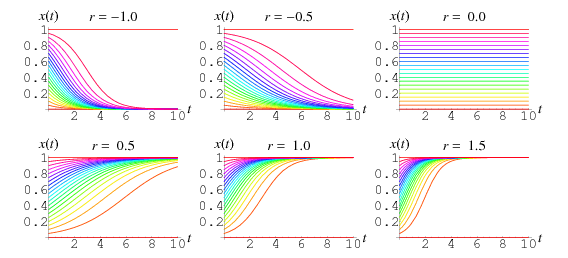
\includegraphics[scale=0.5]{./img/LogisticEquation.png}
    \caption{Logistic Equations}
\end{figure}

\end{enumerate}

